\documentclass[12pt,a4paper]{article}
\usepackage[utf8]{inputenc}
\usepackage[english]{babel}
\usepackage{amsmath}
\usepackage{amsfonts}
\usepackage{amssymb}

\usepackage{graphicx}
\usepackage{caption}
\usepackage{subcaption}

\usepackage{hyperref}

\author{Sven Eriksson}
\title{Writeup for Advanced Lane Finding Project \\ \large{Part of Udacity self driving car nanodegree}}

\setlength{\parindent}{0pt} % Default is 15pt.
\usepackage{parskip}


\begin{document}
\maketitle

\section*{The goals / steps of this project are the following}
\begin{itemize}
\item Compute the camera calibration matrix and distortion coefficients given a set of chessboard images.
\item Apply a distortion correction to raw images.
\item Use color transforms, gradients, etc., to create a thresholded binary image.
\item Apply a perspective transform to rectify binary image ("birds-eye view").
\item Detect lane pixels and fit to find the lane boundary.
\item Determine the curvature of the lane and vehicle position with respect to center.
\item Warp the detected lane boundaries back onto the original image.
\item Output visual display of the lane boundaries and numerical estimation of lane curvature and vehicle position.
\end{itemize}

I have done all of these things and the purpose of this report is to describe that.

My code is organized in several files:
\begin{itemize}
\item main.py
\item development.py
\item undistort.py
\item transformPerspective.py
\item findLines.py
\item imageFilters.py
\end{itemize}

I used 'development.py' to test my pipeline on the provided test images. Almost every step of the pipeline for every test image can be seen in the folder 'output\_images'.

\section{Camera Calibration}
\subsection{Briefly state how you computed the camera matrix and distortion coefficients. Provide an example of a distortion corrected calibration image.}

By using the openCV function findChessboardCorners I found and localized the internal corners in the chessboard and assigned them to corners on an imagined chessboard on a flat surface.

I then used the localized and imagined corners as input to the openCV function calibrateCamera to get the camera matrix and distortion coefficents.

The code for this operation and the final distortion operation can be found in the file 'undistort.py'. See figure \ref{distorted} for an example of an undistorted image and its original.

\begin{figure}
    \centering
    \begin{subfigure}[b]{0.45\textwidth}
        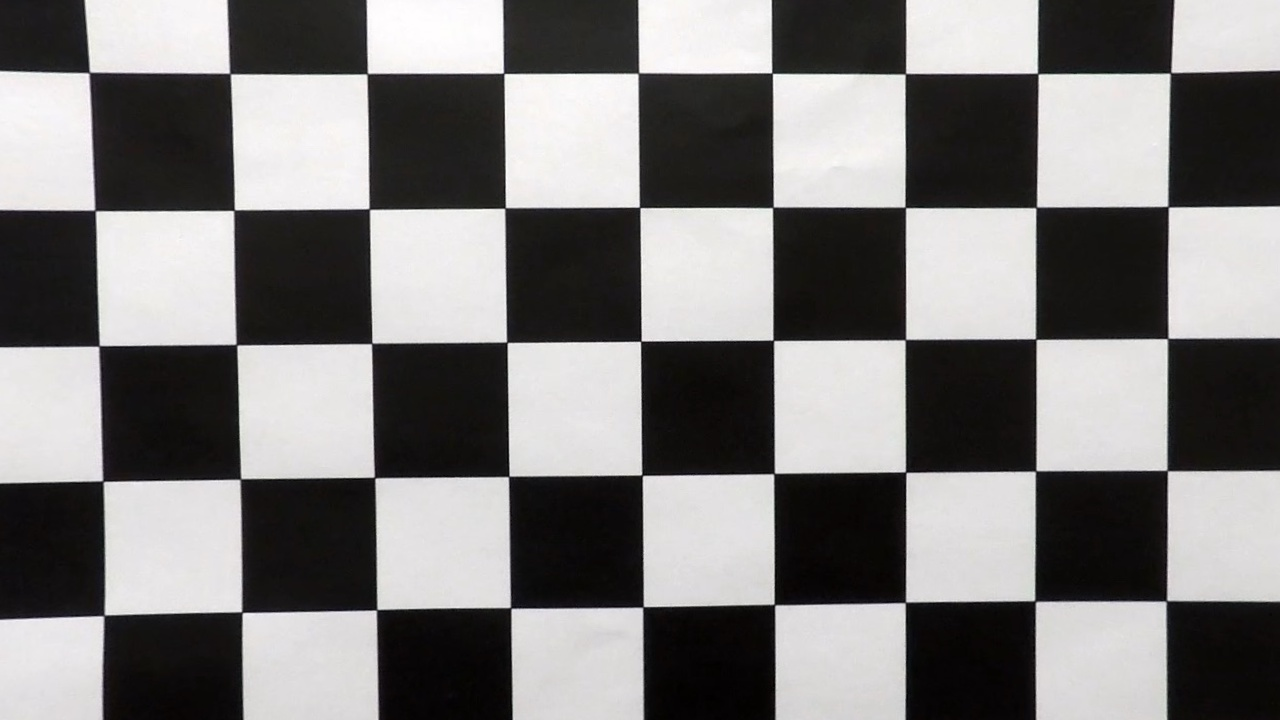
\includegraphics[width=\textwidth]{../output_images/undist-chessboard.jpg}
        \caption{Distortion corrected}
    \end{subfigure}
    \begin{subfigure}[b]{0.45\textwidth}
        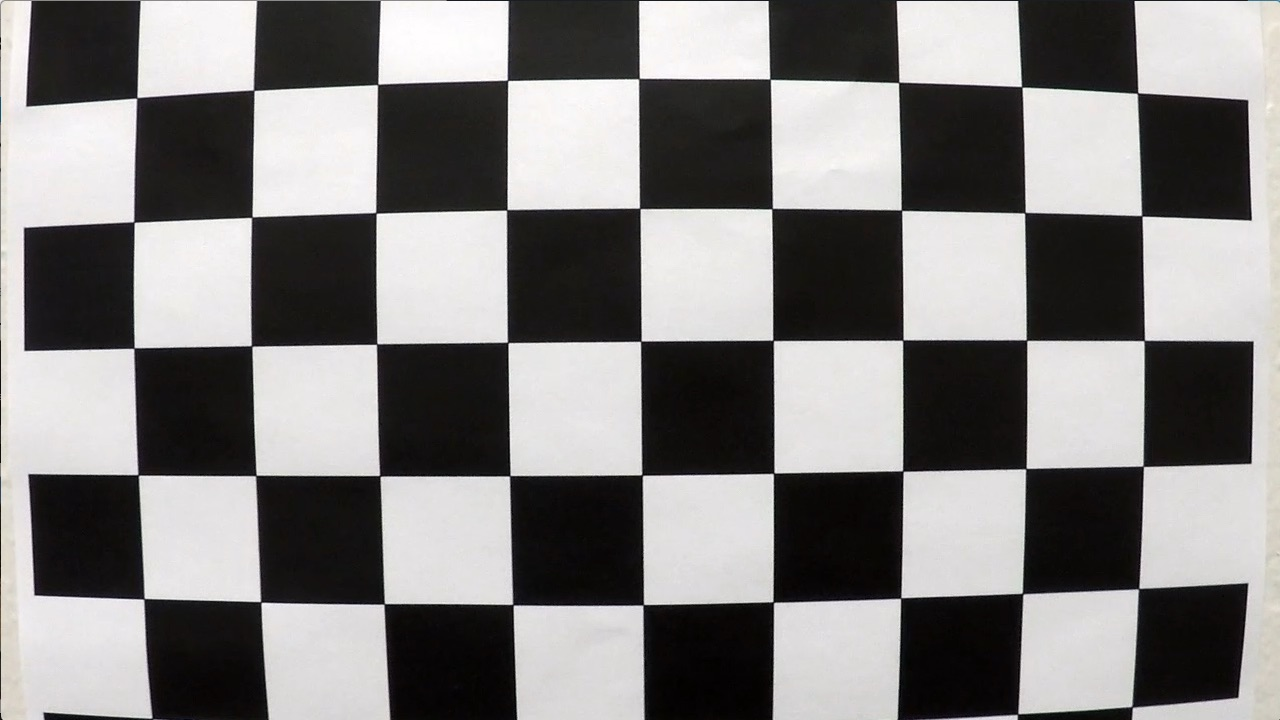
\includegraphics[width=\textwidth]{../camera_cal/calibration1.jpg}
        \caption{Original}
    \end{subfigure}
    \caption{An undistorted chessboard and the orignal image.}
    \label{distorted}
\end{figure}

\section{Pipeline (single images)}


\subsection{Provide an example of a distortion-corrected image.}

See figures \ref{distorted} and \ref{distorted_road}.

\begin{figure}
    \centering
    \begin{subfigure}[b]{0.45\textwidth}
        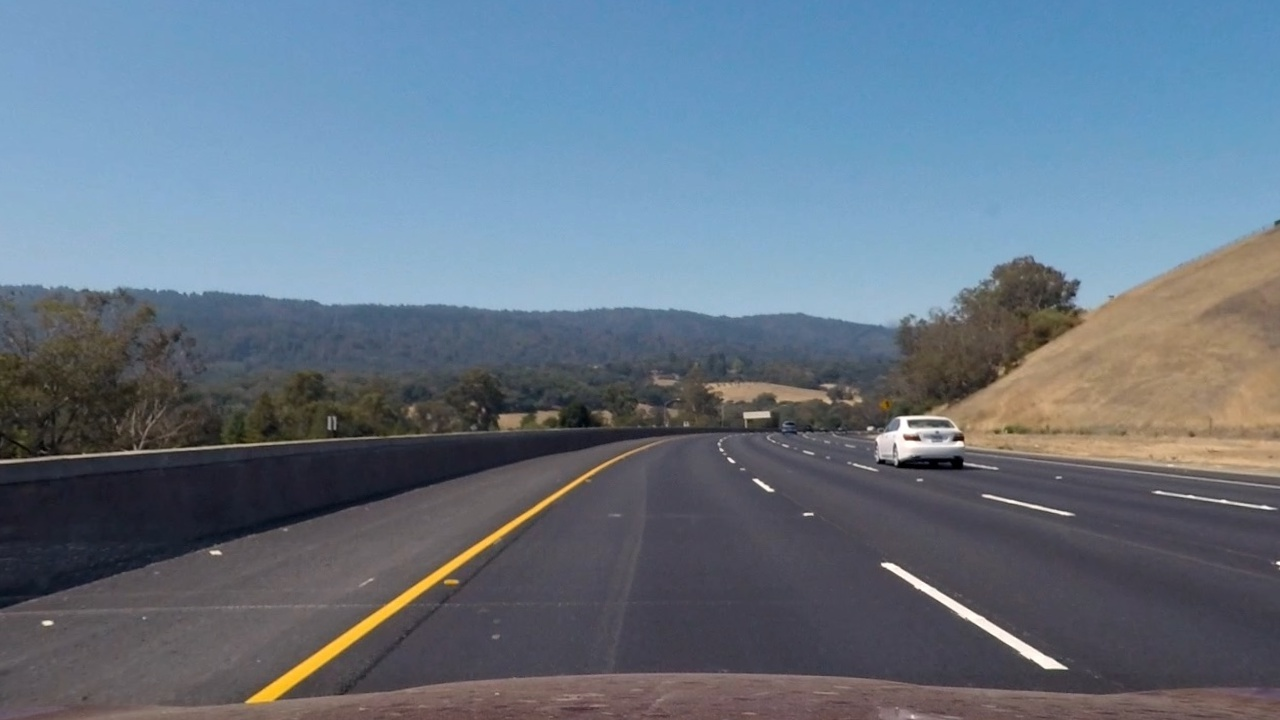
\includegraphics[width=\textwidth]{../output_images/undist-test3.jpg}
        \caption{Distortion corrected}
    \end{subfigure}
    \begin{subfigure}[b]{0.45\textwidth}
        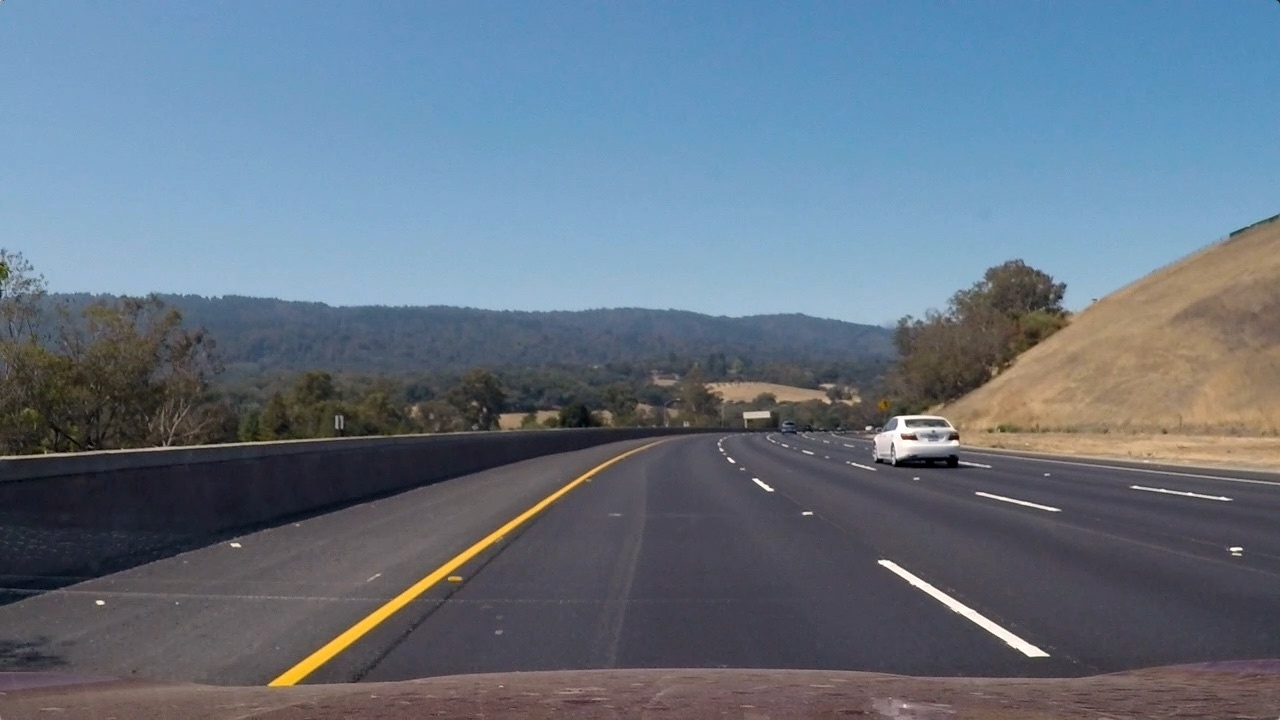
\includegraphics[width=\textwidth]{../output_images/original-test3.jpg}
        \caption{Original}
    \end{subfigure}
    \caption{An undistorted road picture and the orignal image.}
    \label{distorted_road}
\end{figure}

\subsection{Describe how (and identify where in your code) you used color transforms, gradients or other methods to create a thresholded binary image.  Provide an example of a binary image result.}
The code for creating a thresholded binary image is located in 'main.py'. It is also located in 'development.py' for testing settings on the provided test images. 'main.py' contains the final pipeline adapted for video.

I am using the sobel operator in both X and Y directions as thresholds. I do also combine these two to use the combined magnitude and the direction as thresholds.

I addition to the sobel operator I do also use threshold based on the HLS colorspace where I use hue and saturation. I use two separate thresholds for hue. One for white and one for mostly yellow.

I combine these 7 thresholds by requiring that each pixel that is marked as a lane line in 6 or more shall be considered a lane line in my combined threshold. See figure \ref{threshold} for an example.

\begin{figure}
  \centering
    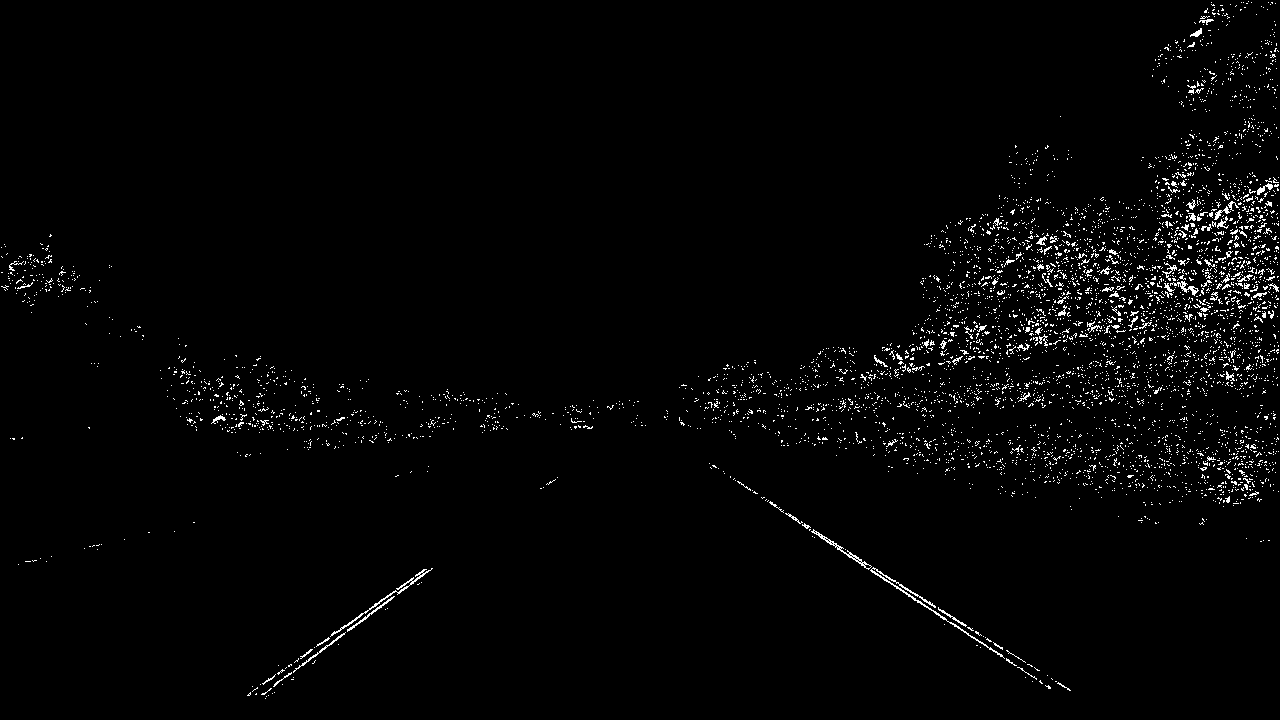
\includegraphics[width=0.5\textwidth]{../output_images/combined-straight_lines2.png}
    \caption{Combination of my 7 thresholds for the image 'straight\_lines2.png'. At each white pixel at least 6 thresholds were forfilled.}
    \label{threshold}
\end{figure}

\subsection{Describe how (and identify where in your code) you performed a perspective transform and provide an example of a transformed image.}
The perspective transformation is done within the file 'transformPerspective.py'.

I used the following 4 points in the normal perspective and bird perspective. The two openCV functions getPerspectiveTransform and warpPerspective was used.

\begin{tabular}{| l | l |}
\hline
Normal & Bird \\
\hline
213, 690 & 200, 720 \\
590, 450 & 200, 720 \\
690, 450 & 1080, 720 \\
1067, 690 & 1080, 720 \\
\hline
\end{tabular}

See figure \ref{perspective} for an example.

\begin{figure}
    \centering
    \begin{subfigure}[b]{0.45\textwidth}
        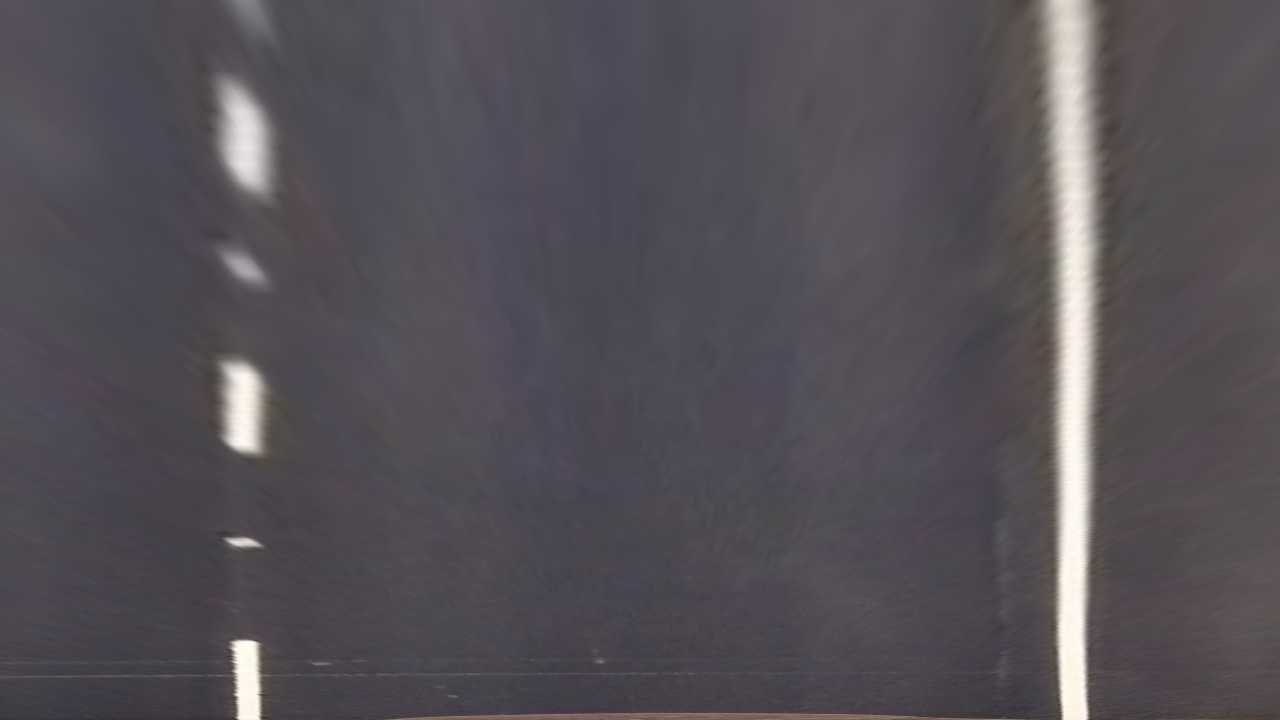
\includegraphics[width=\textwidth]{../output_images/transformed-straight_lines2.jpg}
        \caption{Bird perspetive distortion corrected original.}
    \end{subfigure}
    \begin{subfigure}[b]{0.45\textwidth}
        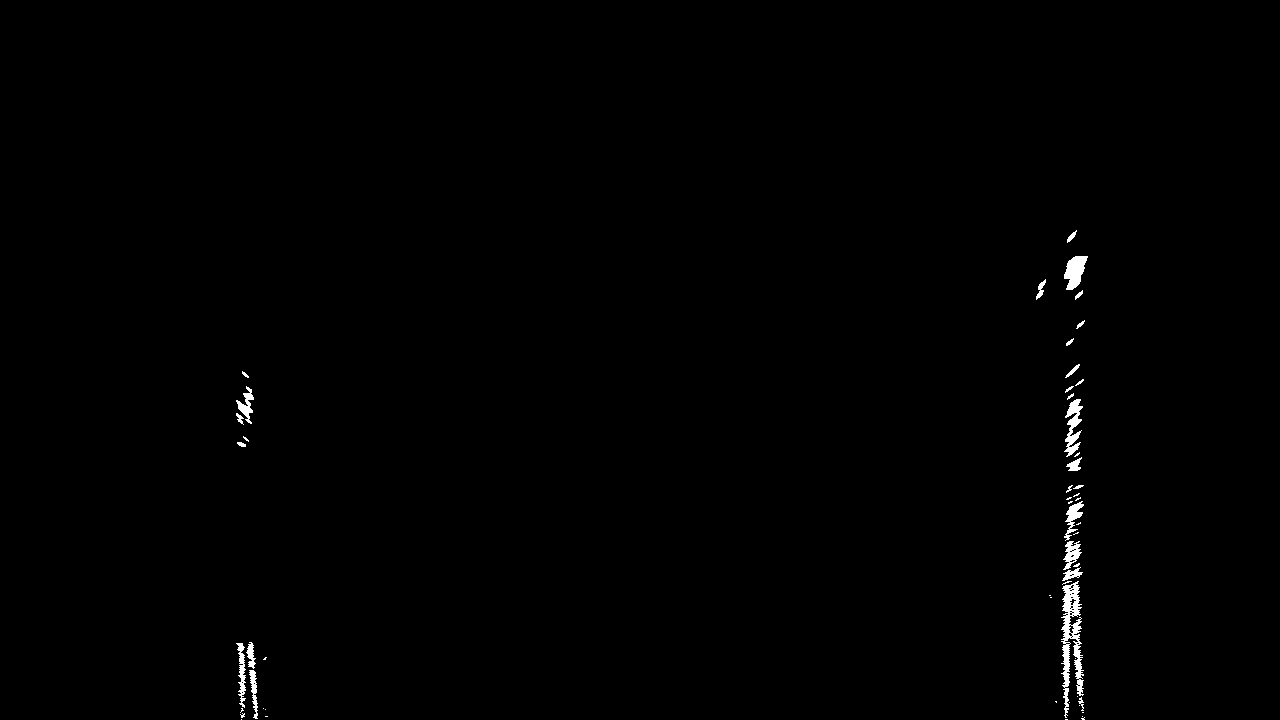
\includegraphics[width=\textwidth]{../output_images/combinedAndTransformed-straight_lines2.png}
        \caption{Bird perspective of thresholds.}
    \end{subfigure}
    \caption{Perspective transform of 'straight\_lines2.png'. This is the same picture as shown in figure \ref{threshold}}
    \label{perspective}
\end{figure}


\subsection{Describe how (and identify where in your code) you identified lane-line pixels and fit their positions with a polynomial?}
The identification of lane-line pixels on a perspective transformed threshold image is done within the file 'findLines.py'.

As can be seen in figure \ref{perspective}. My thresholds keeps the line and little else. Unfortunatly it does sometimes also filter out most of the line. 

I divided the transformed threshold image in a left and right half and assigned all points in the right half to the right line and all points in the left half to the left line. This is possible due to the fact that I rarely have anything else than the lines in these images.

Due to the fact that sometimes there was only a small part of a line left I decided to assume that the lines were parallel and implemented my own polynomial fit function. This can be found at row 16 - 26 in the file 'findLines.py'.


\subsection{Describe how (and identify where in your code) you calculated the radius of curvature of the lane and the position of the vehicle with respect to center.}
The curvature and position with respect to center is also calculated in the file 'findLines.py'.

Curvature is calculated within a function at row 29. I multiply the pixel values by distance in the real world per pixel and repeats the polynomial fit function. Then I use the coefficients from my polynomial to calculate a radius estimation. My radius estimation for the first curve seem to be in the range of 300-500m and I would argue that it is within the same order of magnitude as 1km.

\subsection{Provide an example image of your result plotted back down onto the road such that the lane area is identified clearly.}
See figure \ref{resultMappedToRoad}.
\begin{figure}
  \centering
    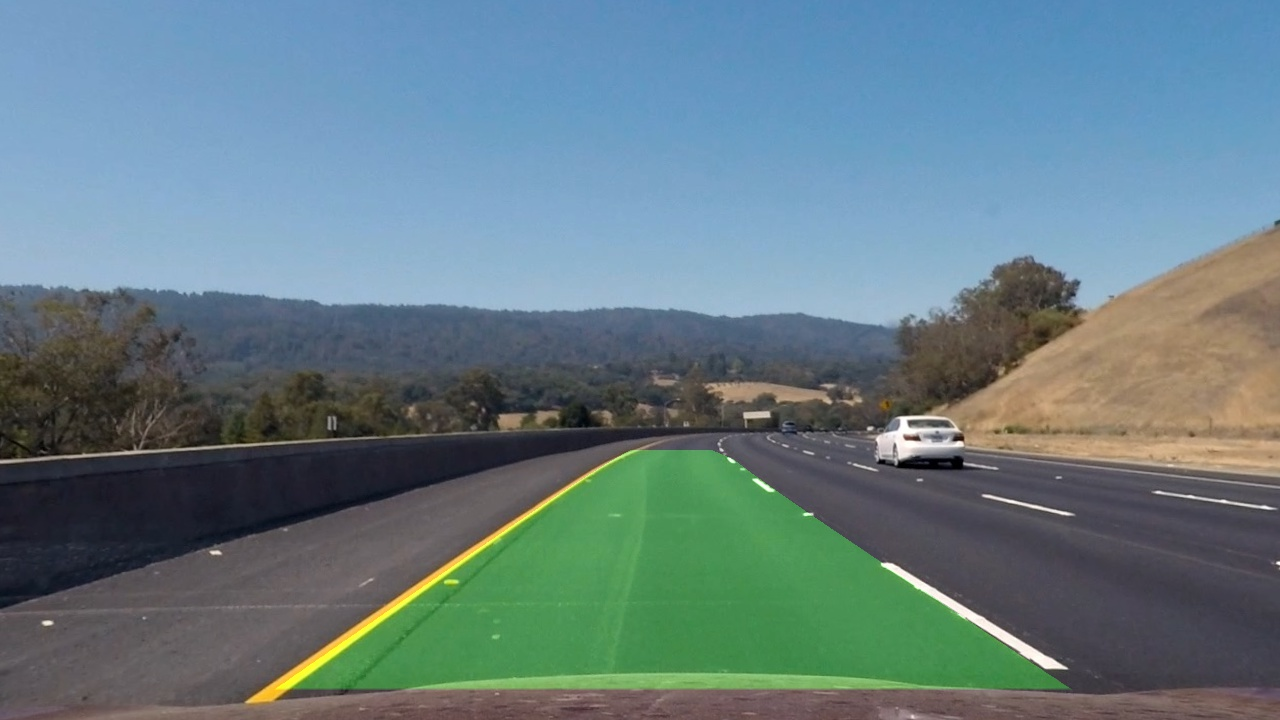
\includegraphics[width=0.5\textwidth]{../output_images/resultWithLines-test3.jpg}
    \caption{This is the result of the pipeline for the image 'test3.jpg'.}
    \label{resultMappedToRoad}
\end{figure}


\section{Pipeline (video)}

\subsection{Provide a link to your final video output.  Your pipeline should perform reasonably well on the entire project video (wobbly lines are ok but no catastrophic failures that would cause the car to drive off the road!).}
The final output is located at:

\url{http://svene.se/carND/laneLines.mp4}

\section{Discussion}
\subsection{Briefly discuss any problems / issues you faced in your implementation of this project.  Where will your pipeline likely fail?  What could you do to make it more robust?}
While removing everything but the lines in my thresholds simplified the polynomial fit I did sometimes remove the entire line and did then have to rely on previous polynomial fits. The condition for detecting such a failure will likely make this process less reliable on other roads.

So I should try to remove less off the line through my thresholds while still not getting to much noise. One option is to implement the recomended sliding window search that I did not use due to having to few points in some images.

\end{document}